\documentclass[a4paper,10pt]{scrartcl}
\usepackage[ngerman]{babel}
\usepackage[T1]{fontenc}
\usepackage[utf8]{inputenc}
\usepackage{graphicx}
\usepackage{float}

\title{Datenbanken 1}
\author{Benjamin Altmiks}
\date{10. Oktober 2018 - \today}
\begin{document}
\maketitle
\tableofcontents
\newpage
\section{Einleitung}
\subsection{Grundlagen und Basiskonzepte}
\subsubsection{Motivation}

\begin{itemize}
    \item Mehrbenutzerbetrieb
    \item Transaktionen (Deadlock Vermeidung) 
    \item Anweisungsorientiert (Eine Anweisung ganz oder gar nicht)
    \item Zugriffsrechte und Zugriffsmöglichkeiten
    \item Sicherungsmechanismus
\end{itemize}
\subsubsection{Datenbanken Terminologie}
\textbf{a) Daten}\newline
Daten sind Zeichen, die zum Zweck der Verarbeitung Informationen aufgrund bekannter oder unterstellter Abmachungen (Interpretationsregeln) darstellen.\newline
\textbf{b) Datensatz}\newline
Ein Datensatz ist eine logische Zusammenfassung von Daten zu einer Einheit.\newline
\textbf{c) Datenbank}\newline
Eine Datenbank (DB) ist ein integrierter, persistenter Datenbestand einschließlich aller relevanten Informationen(Metainformation)\newline
\textbf{d) Systemkatalog}\newline
Ein Verwaltungsinformationsrechner, der physische und logische Datenbankbearbeitung verwaltet. (Data Dictonary)\newline
\textbf{e)Datenbankverwaltungssystem(DBVS/DBMS)}\newline
Die Gesamtheit aller Programme zum verwenden einer Datenbank\newline

Eine Datenbank besteht aus einem Datenbestand und seinem Systemkatalog und kann über ein DBMS im Datenbanksystem verwendet werden.
\begin{figure}[h]
	\centering
	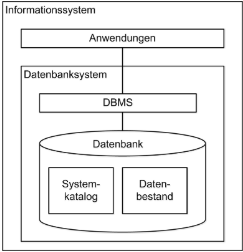
\includegraphics[width = 0.3\textwidth]{Grundaufbau.PNG}
	\label{img:grafik-dummy}
\end{figure}

\subsection{Architektur eines DBMS}
\subsubsection{3.Schema-Architektur (ANSI/SPARC)}
Besteht aus den drei Ebenen
\begin{itemize}
    \item Die externe Ebene = Struktur der Daten
    \item Die konzeptionelle Ebene = beschreibt den relevanten Informationsbereich
    \item Die interne Ebene = physische Abspeicherung und die Zugriffsorganisation
\end{itemize}

\subsubsection{Sprachschnittstellen}
\textbf{DML} = data manipulation language (Eintrage, Ändern und Löschen mit Anfrage)\newline
\textbf{DDL} = data definition language (Umsetzung der Strukturen)\newline
\textbf{DAL} = data administration language (Soeicherorganisation, Strukturumsetzung)\newline

\subsection{Datenmodell (DM)}
Ein formales Konzept der Beschreibung von Datenbankstrukturen
\begin{figure}[h]
	\centering
	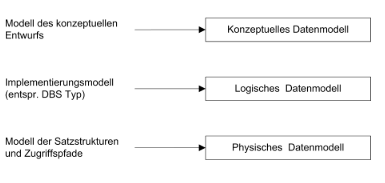
\includegraphics{Datenmodelle.PNG}
	\label{img:grafik-dummy}
\end{figure}

\subsubsection{Ebenen}
\textbf{Konzeptuelle Ebene}\newline
Beschreibungsmodell für Informationsstrukturen mit graphischer Notation
\newline\textbf{Logische Ebene}\newline Implementierungssicht, d.h Herleitung aus dem konzeptuellen Datenmodell 
\newline\textbf{Physische Ebene}\newline Verteilung der Daten auf Platen, also physische Speicherstrukturen
\subsubsection{Datenmodell-Typen} 
Satz- bzw. Tupelorientierte Beschreibungstechniken bei klassischen DM.\newline
Im Gegensatz dazu semantische DM mit Objekt- bzw. infromationsorientiert
\newline\textbf{Semantisches Datenmodell}\newline
Eine abstrakte, formale Beschreibung und Darstellung von Infromationen. Weitere Zerlegung der Darstellung nicht möglich (semantisch irreduzibel). Es zeigt die Beziehungen mithilfe von Modellierungskonstrukten dar.
\newline\textbf{Relationales Datenmodell} \newline
Ist die Darstellung von Datensätzen mithilfe von mathematischen Tabellen
\newline\textbf{Objektdatenmodell}\newline
Ein objektorientiertes Datenbankmodell verfolgt den Ansatz, Daten zusammen mit ihren Funktionen in einem Objekt zu speichern.
\section{Modellierung}
Zum Übertragen von Daten ist es notwendig Information und Interpretationsregeln festzulegen. Erst dann kann eine Infromationsanalyse durchgeführt werden.  
\subsection{Objekte und Analyse}
\subsubsection{Objekt- und Assoziationstyp}
Ein Objekttyp repräsentiert die Menge aller Objekte, die die gleiche klassifizierende Bedingung erfüllen. 
Objekttypen enthalten nur unterschiedliche Objekte. Das selbe gilt für Assoziationstypen (Beziehung).
\subsubsection{Rolle und Mitgliedschaft}
Die Rolle beschreibt den Beitrag eines Objekttypen zum Informationsgehalt eines Assoziationstypen. Ein Mitgliedschaftsintervall m:n (m: Untergrenze, n:Obergrenze) r bedeutet, dass ein Objekt des betreffenden Typs in mindestens m Assoziationen des Assoziationstyps auftreten muss bzw. in höchstens n Assoziationen auftreten darf.
\subsection{System-/Basistypen}
Systemtypen stellen die Domänen des Systems dar. Alle möglichen Werte der Domänen sind Objekte des Systemtypen. 
Systemtypen sind Objekttypen. (String, Boolean)\newline  
Eine \textbf{Repräsentation} liegt vor, wenn ein Objekt durch ein Zeichen repräsentiert werden kann.  
\textbf{Basistypen} sind Objekttypen, die durch einen Systemtypen repräsentiert werden und alle Objekte aus dem Systemtypen übernehmen.
\subsection{Dreiecksbeziehung}
Ein Assoziationstyp ist eine benannte Beziehung zwischen n Objekttypen (n >= 2), die in dieser Beziehung bestimmte Rollen spielen.

\subsection{Vererbung}
Ein Objekttyp ist Untertyp eines anderen Objekttypen (Obertyp), wenn alle Objekte des Untertypen eine Teilmenge des Obertypen bilden. Man Unterscheidet zwischen verschiedenen Beziehungen zwischen Untertypen.
\begin{itemize}
    \item \textbf{or} = Die Untertypen können eine Schnittmenge haben
    \item \textbf{xor}= Die Untertypen sind gegenseitig exklusiv
    \item \textbf{and} = Die Untertypen haben dieselben Objekte
\end{itemize}












\end{document}
